\newpage
\chapter*{Themes}
\addcontentsline{toc}{chapter}{4. Themes}
% Chapter for each research question
% how we validated it and proved it worked

A theme is a governed template. Unlike with templates, themes are written using \gls{CSS}. The \gls{CSS} manages the presentation, and graphical layout of a web page. A theme specifies the fonts, font sizes, layout of text, colour scheme, and related imagery. 

Themes should be independent from the content of a website. This is so that a theme can be changed without affecting the content, causing a developer to rewrite the content. 

There are currently two themes to use with Taylor'd UI, a material design theme, and a flat modern theme. The themes are built on top of the Taylor'd UI framework, and are to be used in conjunction with the framework.

The material design theme follows the google guidelines on styles \citep{Google17}. The colours are kept to muted tones of primary colours. The font is changed to Google's Roboto for the primary font choice, and Nunito as the secondary font.

When using the material design theme, the font sizing also changes to be in line with Google's styles. In keeping with the style, a small drop shadow was also added to assets such as buttons as seen in Figure.~\ref{fig:temtheme} on  page~\pageref{fig:temtheme}

Instead of having the generic placeholder images that are found in the templates as seen in Figure.~\ref{fig:gentemp} on  page~\pageref{fig:gentemp}, random creative common images are taken from unsplash.com as using the unsplashit service \citep{SPL17}. 

The modern theme is similar to the material design theme, in keeping the theme understated. This theme does however has more modern, and interesting font choices such as Raleway. 

A theme can be added to any of the templates by creating a link to the stylesheet as seen below.

\begin{lstlisting}[language=HTML]
 <link rel="stylesheet" href="../../assets/css/taylord.css" />
\end{lstlisting}

\begin{figure}[h]
\centering
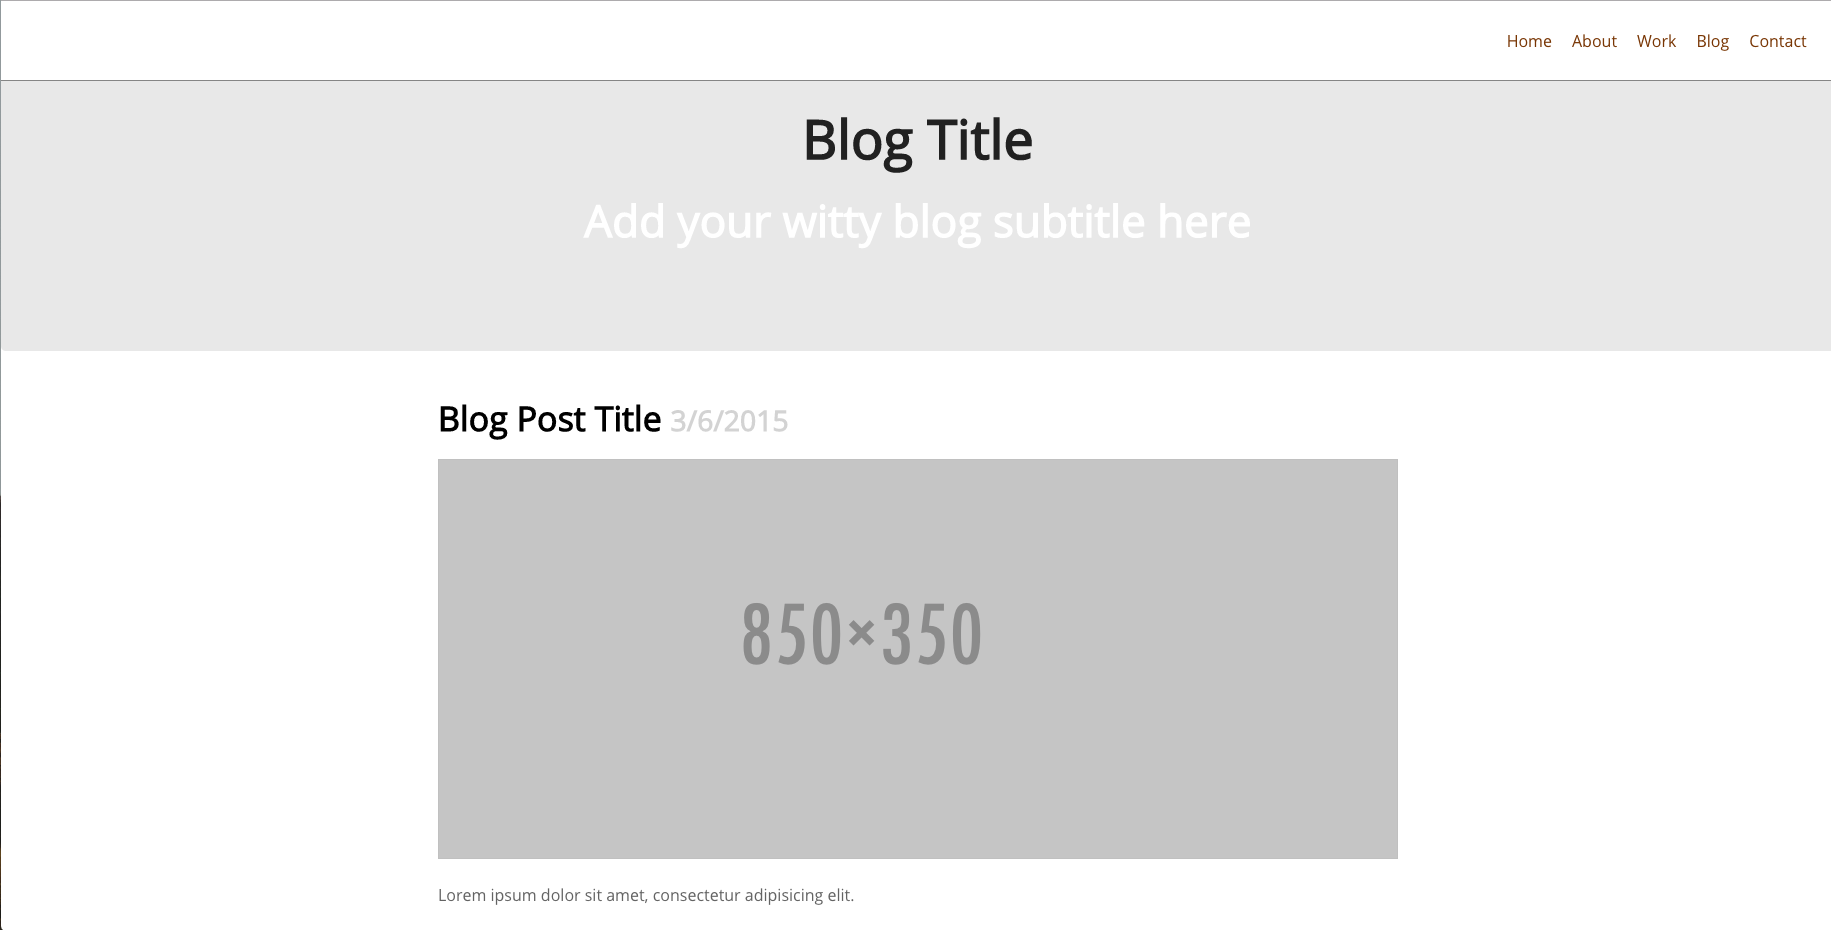
\includegraphics[scale=0.13]{images/placeholderTemp}
\caption{Generic Template}
  \label{fig:gentemp}
\end{figure}


\begin{figure}[ht]
\centering
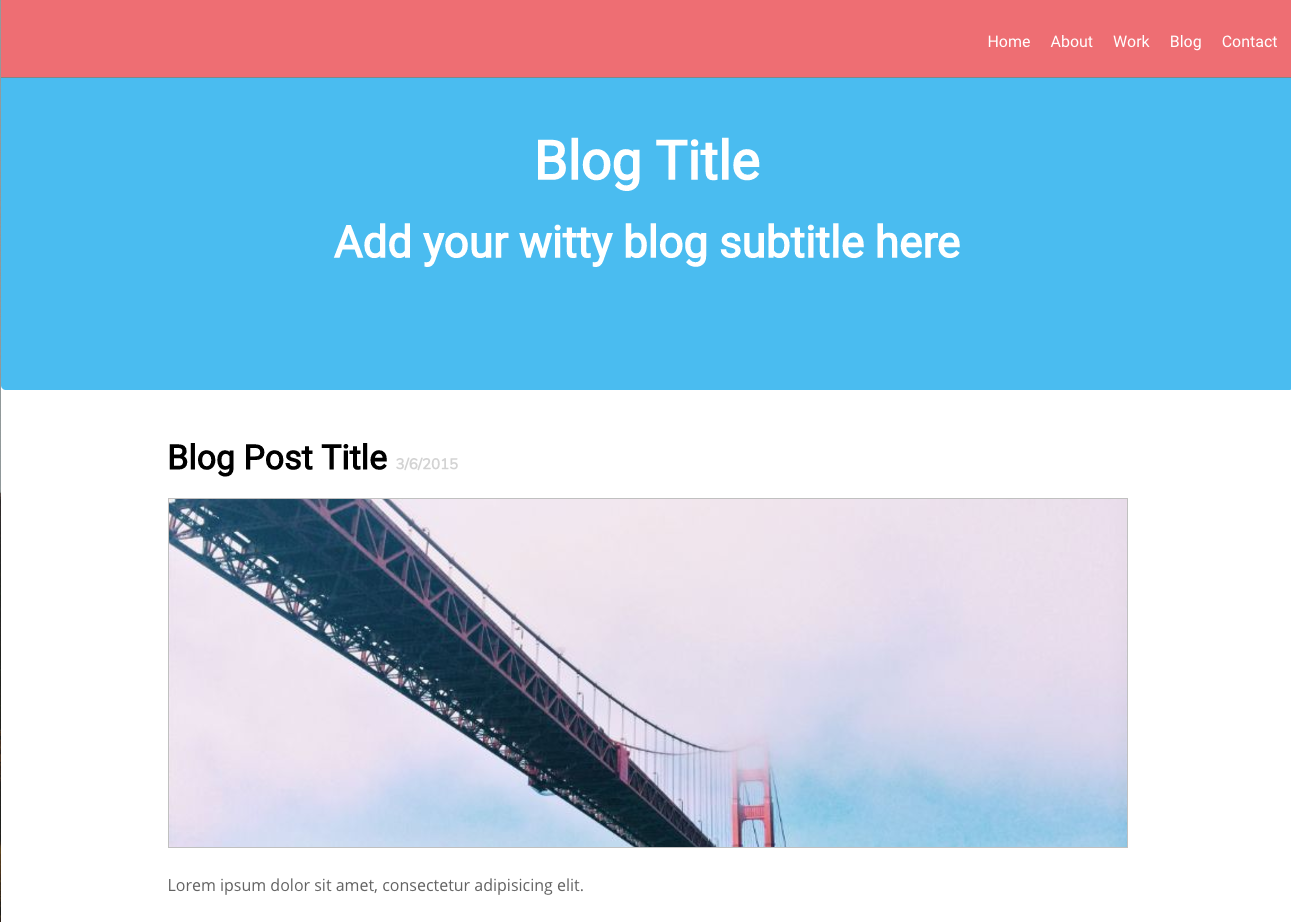
\includegraphics[scale=0.2]{images/withtheme}
\caption{Template with theme}
  \label{fig:temtheme}
\end{figure}

